\chapter{Implementation}

\section{Introduction}
This chapter details the implementation phase of our project, which follows an agile methodology with four sprints. Each sprint focuses on delivering specific features and functionality according to the project backlog. The implementation utilizes a modern tech stack consisting of React \cite{ReactWebsite} with Vite \cite{ViteJSWebsite} for the frontend, Node.js \cite{NodeJSWebsite} with Express.js \cite{ExpressJSWebsite} for the backend, MySQL \cite{MySQLWebsite} for database management, and Tailwind CSS \cite{TailwindWebsite} for styling.

Our first sprint focused on establishing essential foundational components of the system, with the following key deliverables:

\subsection{Web Backoffice Authentication}
\begin{itemize}
    \item Admin dashboard login and authentication system
    \item Role-based access control for backoffice users (Super Admin, Admin, Agent)
    \item User management interface for creating and managing user accounts
    \item Permission management system for different user roles
    \item Security logs and audit trails for backoffice activities
    \item Session management and secure token handling
\end{itemize}

\subsection{Data Collection and Scraping}
The first sprint also included the development of robust data collection systems focused on gathering real estate market data. These systems were designed to autonomously collect, validate, and store property listings, market trends, and other relevant information from various online sources. This data forms the foundation for the AI-driven features discussed in Chapter 4, including property valuation models and recommendation systems.

\section{Sprint 1: Authentication and User Management}
\subsection{Overview}
The first sprint focuses on establishing the core authentication system and user management functionality. This foundation is critical for all subsequent features as it defines user roles and access controls.

\subsection{User Types}
The system supports three distinct user types, each with different permissions and capabilities:
\begin{itemize}
    \item \textbf{Super Admin}: Has complete access to all system features and can manage admins and agents.
    \item \textbf{Admin}: Can manage agents and has access to administrative features within their assigned scope.
    \item \textbf{Agent}: Has limited access to the system based on their assigned responsibilities.
\end{itemize}


\subsection{Authentication System}
\subsubsection{Sign-up Process}
The sign-up process is illustrated in Figure \ref{fig:signup-diagram} below. The diagram shows the authentication flow for new users registering in the system.

\begin{figure}[ht!]
    \centering
    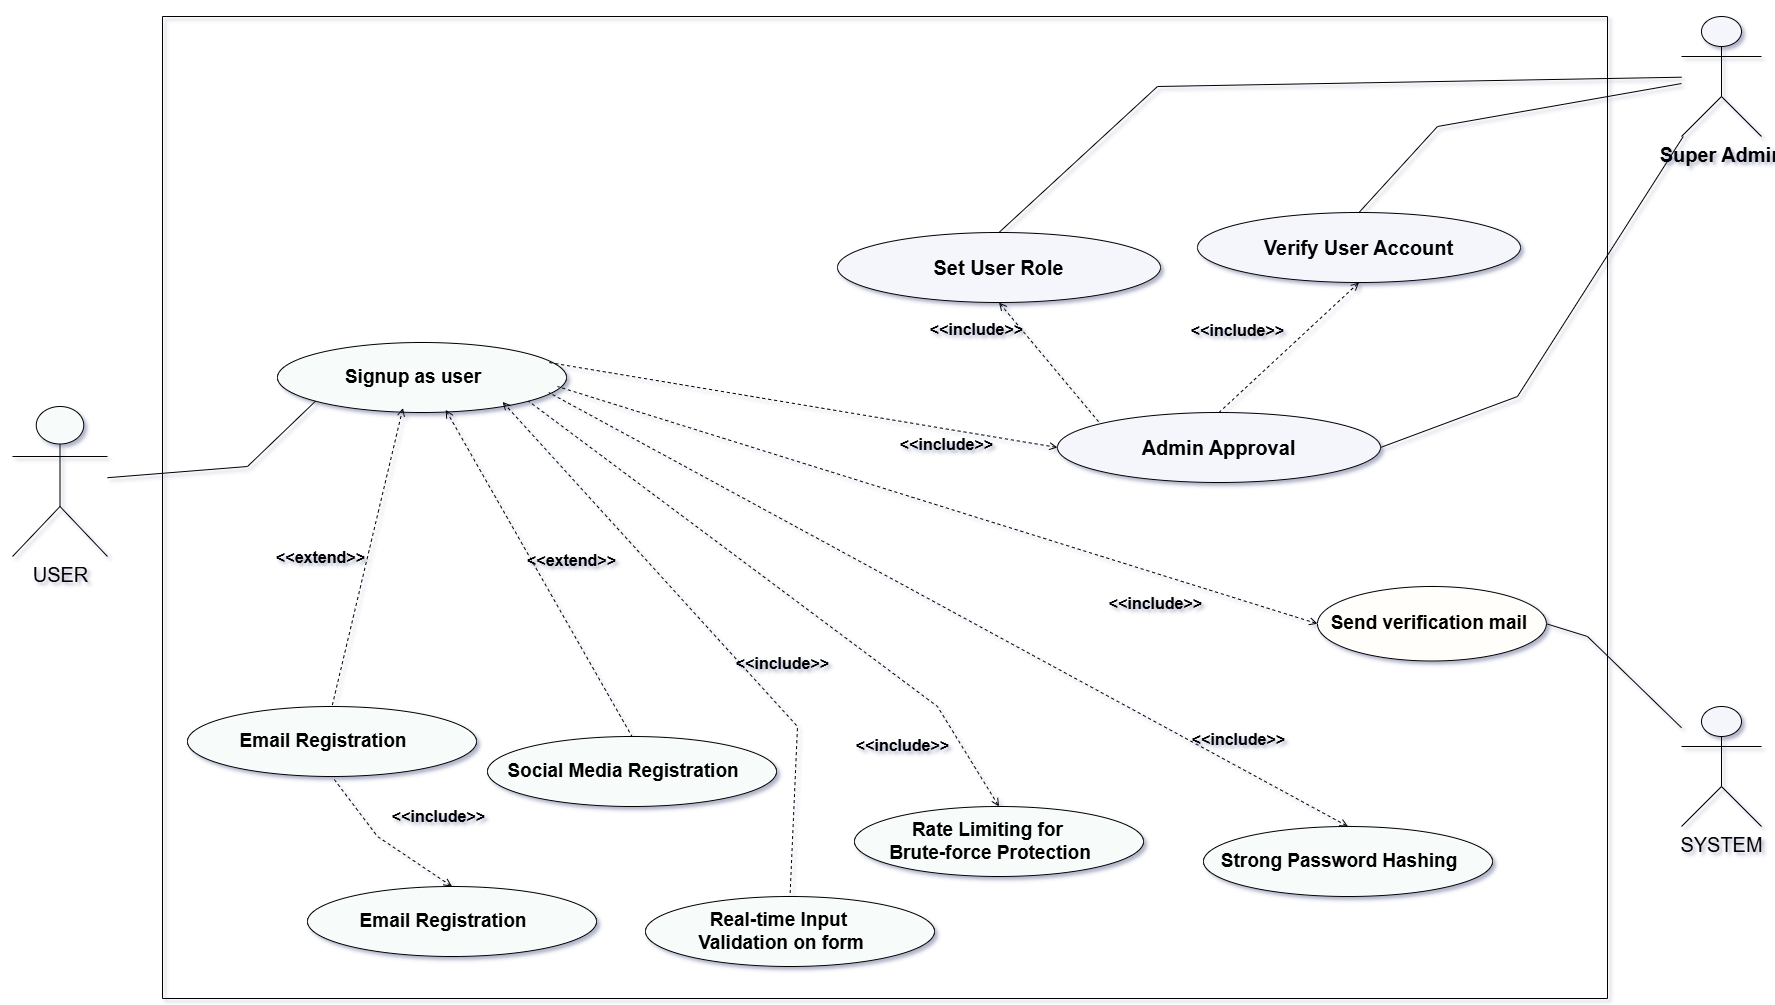
\includegraphics[width=1\textwidth]{images/diagram_de_case_d_utilisation_signup.png}
    \caption{Authentication Sign-up Use Case Diagram}
    \label{fig:signup-diagram}
\end{figure}

% \vspace{1cm}


The sign-up process includes user registration, role assignment, and account verification steps. During registration, users are categorized into one of the three user types: Super Admin, Admin, or Agent, with each type having different permissions and access levels within the system.

\section{Data Collection and Scraping}
\subsection{Overview}
This section details the data collection processes implemented to gather the real estate market data required for our AI models. Effective data acquisition is a critical foundation for the AI capabilities described in Chapter 4.

\subsection{Real Estate Data Scraping}
\subsubsection{Data Sources}
We implemented automated scraping systems to collect real estate data from various sources:
\begin{itemize}
    \item Real estate listing websites such as PropertyStar Tunisia \cite{PropertyStarTunisia} for comprehensive property listings and pricing data
    \item Property transaction records from public databases
    \item Real estate market reports and analytics platforms
    \item RE/MAX Tunisia \cite{RemaxTunisia} for detailed property valuation data in both sale and rental markets
    \item Al-Mindhar \cite{AlMindhar} for blog content related to legal aspects, investment strategies, and real estate regulations in Tunisia to train knowledge-based AI assistants
\end{itemize}

\subsubsection{Scraping Architecture}
\begin{figure}[ht!]
    \centering
    % Placeholder for a diagram of the scraping workchart
    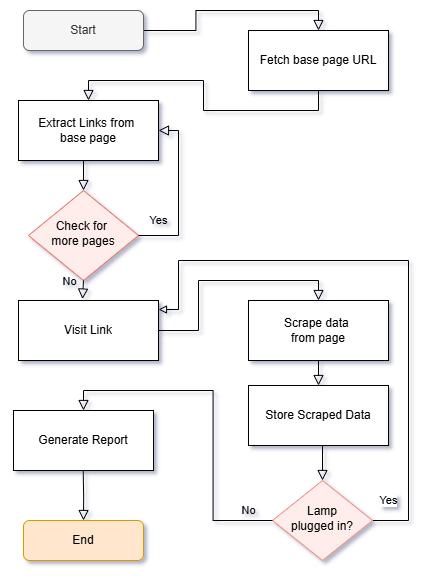
\includegraphics[width=1\textwidth]{images/workchartscraper.png}
    \caption{Data Scraping workchart}
    \label{fig:scraping-workchart}
\end{figure}

Our scraping system uses a distributed architecture with the following components:
\begin{itemize}
    \item Rate-limiting and request throttling to respect website policies
    \item Scheduled jobs for regular data updates
    \item Data validation and cleaning pipelines
\end{itemize}

\subsection{Data Storage and Management}
\subsubsection{Database Schema}
The collected data is stored in a structured database with the following key entities:
\begin{itemize}
    \item Property listings (with pricing history)
    \item Location data (neighborhoods, cities, regions)
    \item Property features and amenities
    \item Transaction records and market trends
\end{itemize}

\subsubsection{Data Versioning and Updates}
To maintain data quality and currency, we implemented:
\begin{itemize}
    \item Automated data refresh cycles for each source
    \item Version control for dataset updates
    \item Conflict resolution for data from multiple sources
    \item Data quality monitoring and alerting
\end{itemize}

% Additional sections for subsequent sprints will be added later 